\section{Population Generation}

After the terrain has been generated, the user is provided with a tool that lets them mark areas on the terrain where they want cities to be generated.
When one or more markers are placed, they will remain in their designated positions until interacted with by the user, or when the user presses the \textit{Generate Roads} button.
Each marker can be interacted with by hovering over it, which will turn it red.
Clicking on it will make it yellow, which shows that it is selected (see Figure~\ref{fig:citymarkers}). 

\begin{figure}[h!]
  \centering

  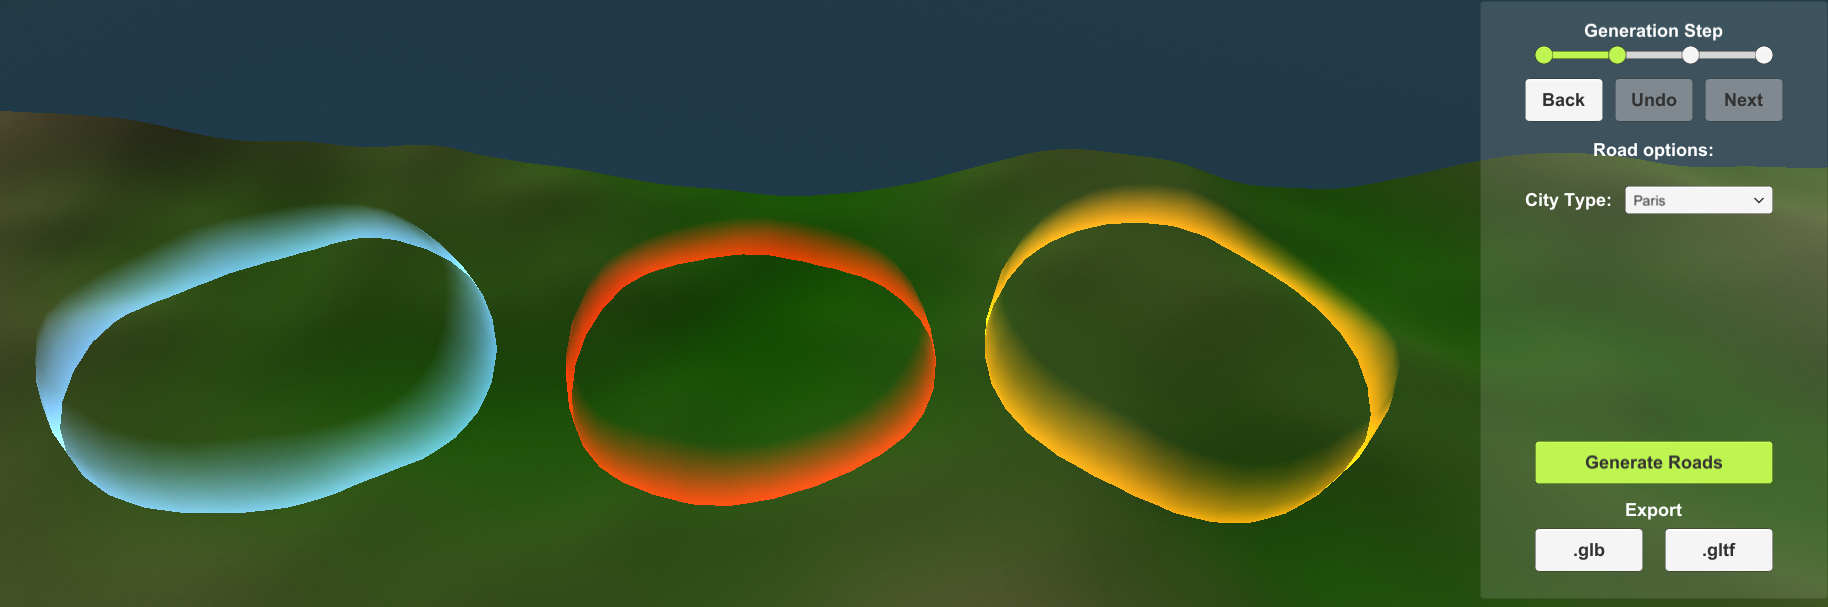
\includegraphics[width=\textwidth]{figure/citymarkers.png}
  \caption{The city marker tool. Each ring represents a potential city, where the radius of the ring roughly corresponds to the size of the city that will be generated.}

  \label{fig:citymarkers}
\end{figure}

\newpage 

Selecting a city marker provides multiple options:
\begin{easylist}
  @ Clicking again and dragging allows the user to freely reposition the marker.
  @ Scrolling up and down increases and decreases the radius of the marker.
  @ Pressing the delete key removes the marker.
  @ Through the menu panel, it is possible to change the type of the city that will be generated. Currently, there are Paris- and Manhattan-style cities available.
\end{easylist}

The population generation begins once the user presses the \textit{Generate Roads} button.
This generates a population density map that covers the entire terrain using a 2-layered Simplex noise function.
Then, the city markers amplify the population of this map, at the spots where they were placed.
Finally, once the population generation is finished, road generation begins.
